\documentclass{article}
\usepackage{KJN}
\usepackage{a4wide,changebar}
\usepackage[numbered,framed]{mcode}

\title{Introduction to Vision and Robotics: Assignment 1}
\author{Chris Swetenham: Student Num, Daniel Mankowitz: S1128165}
\date{3/11/2011}

\begin{document}
\maketitle

\section{Introduction}
\label{sec:introduction}
An overview of the main ideas used in the approach


\section{Methods}
\label{sec:methods}
Describe the vision techniques used

%Detail how these ideas were implemented

%Describe the structure of the code

%How each part is meant to work

%Justify design decisions where appropriate



\subsection{Linking Algorithm}
\label{sec:linking}
The linking algorithm is used to link together detections of a single robot in consecutive frames. Since the images provided in the datasets are RGB, the linking algorithm has been developed to run on each of the three colour channels respectively.\\ 

The algorithm is shown in \figref{fig:link}. Initially, the image on the $k^{th}$ iteration will have been split into three colour channels of red, green and blue respectively. Each colour channel is represented as a separate image and each image has been clipped to a dimension of $120x120$ in the detection algorithm. This enables a more accurate bounding box to be calculated for each robot as there will be less image noise in the clipped image.  \\


\begin{figure}[h!] 
  \centering
    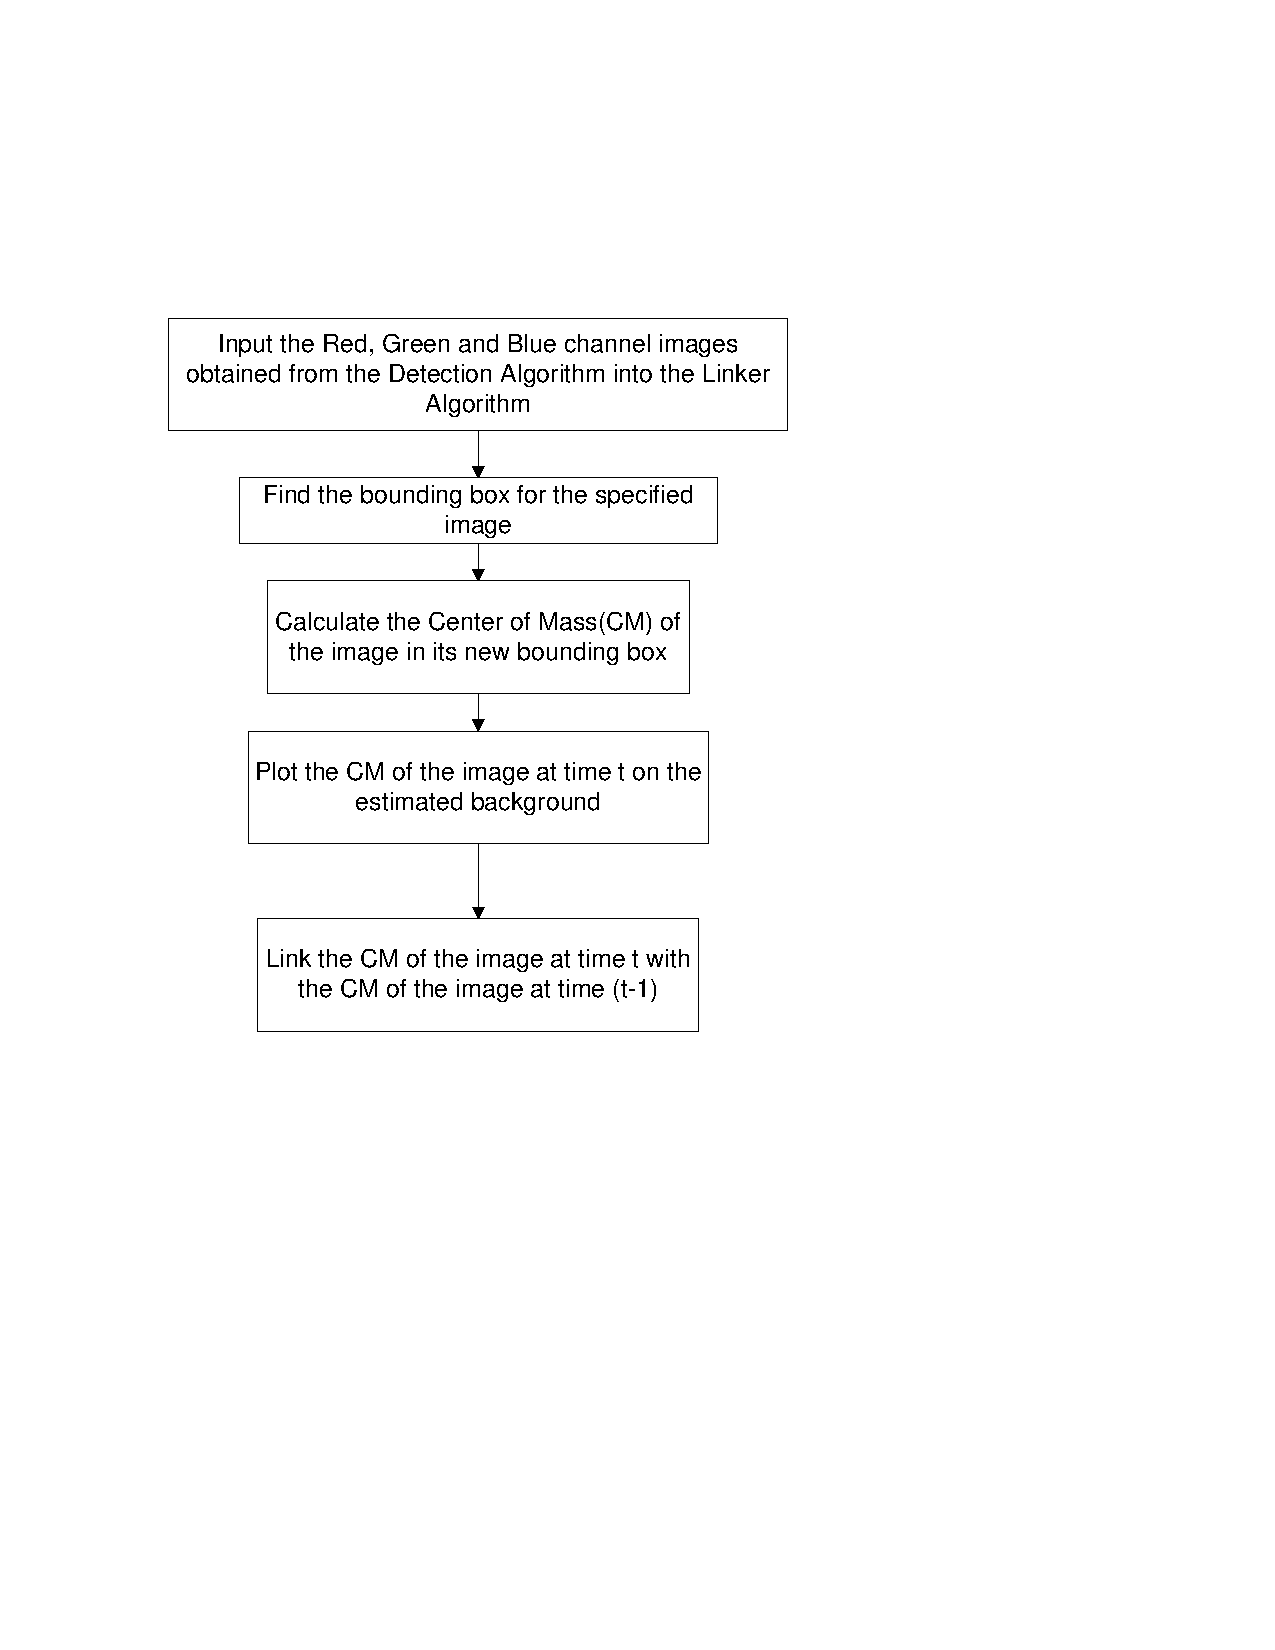
\includegraphics[width=0.5\textwidth]{../Drawings/linkingAlgorithm.pdf}
    \caption{The algorithm developed to link detections of the robot in consecutive frames}
    \label{fig:link}
\end{figure}

\subsubsection{Finding the Bounding Box}
\label{sec:boundbox}

The bounding box of each robot is calculated using the function \textit{calcBoundingBox}. A flow diagram of the function can be seen in \figref{fig:bounding}. This function calculates the bounding box for each robot as well as the box's corresponding centroid in each of the three colour channels respectively.

\begin{figure}[h!] 
  \centering
    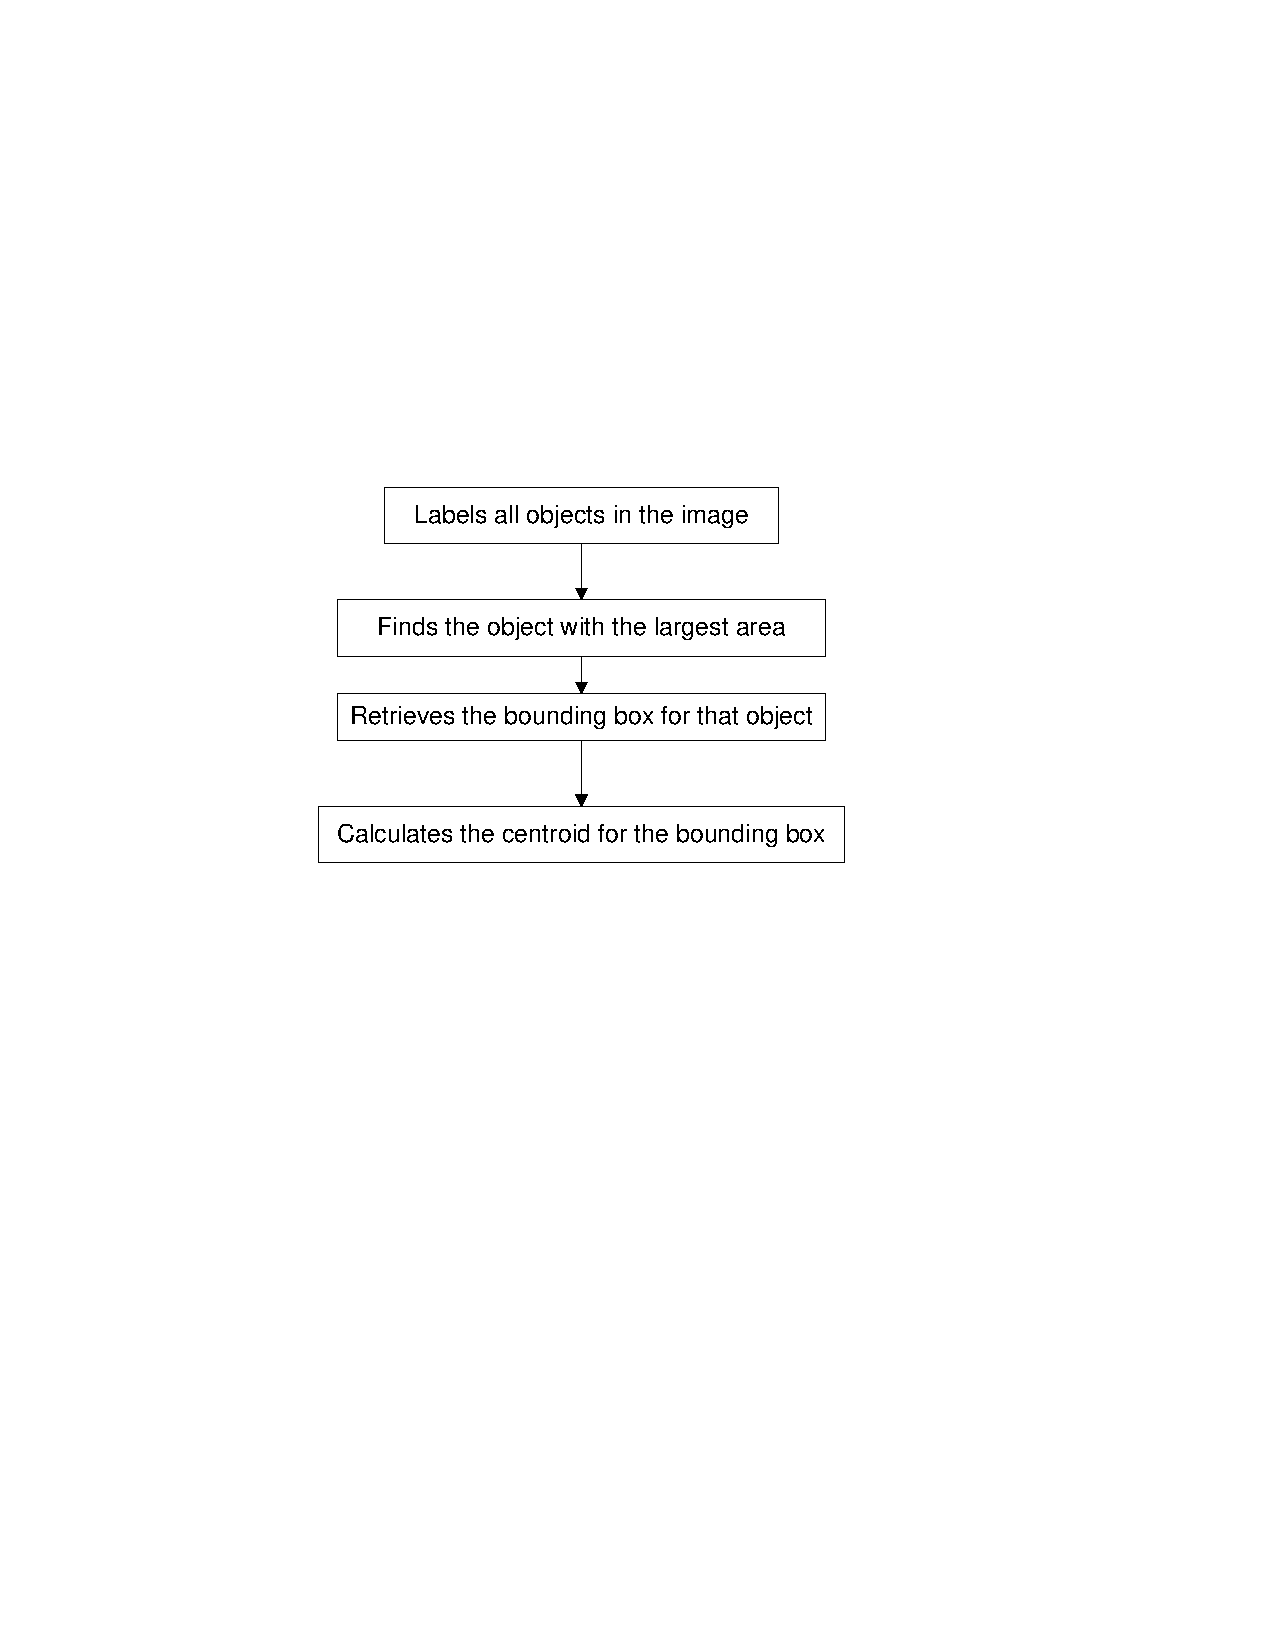
\includegraphics[width=0.5\textwidth]{../Drawings/boundingbox.pdf}
    \caption{The bounding box calculation for each robot }
    \label{fig:bounding}
\end{figure}

An excerpt from the \textit{calcBoundingBox} function is shown below.

\lstinputlisting{calcBoundingBoxReport.m}

Each image is labelled using the \textit{mybwlabel} function as seen in the code excerpt. This will identify all of the objects in the image and assign a set value to each pixel associated with a specific object.  \\

The object with the largest area is then identified. A bounding box is subsequently calculated for the object with the largest area (I.e. the largest number of labelled pixels). This is achieved using the \textit{find} Matlab function which identifies the largest object and stores each pixel belonging to the object with its respective row and column position. This is then used to determine the bounding box of the object.\\

The object will then be surrounded by its corresponding bounding box. The centroid of this bounding box is then calculated. This algorithm is performed on each of the three clipped images corresponding to the three respective colour channels.\\

\subsubsection{Calculate the Center of Mass}
\label{sec:cm}
Once a bounding box for each robot has been determined, the center of mass of the robot needs to be calculated in relation to this new bounding box. This is achieved by utilising the \textit{calcBoundingBoxCM} function.\\

The algorithm initially calculates the area of the object within the bounding box using \eqnref{eqn:area}. This value is used to determine the center of mass of the object within the bounding box.\\

\begin{equation}
A = \Sigma_{r}\Sigma_{c}P_{rc}
\label{eqn:area}
\end{equation}

The center of mass of the object is then determined using \eqnref{eqn:cm}. $(\widehat{r}, \widehat{c})$ are the row and column coordinates of the center of mass of the object respectively.

\begin{equation}
(\widehat{r}, \widehat{c}) = (\frac{1}{A}\Sigma_{r}\Sigma_{c}r P_{rc}, \frac{1}{A}\Sigma_{r}\Sigma_{c}c P_{rc})
\label{eqn:cm}
\end{equation}

\subsubsection{Linking and Plotting}
\label{sec:linkplot}
The final step in the linking algorithm is to link the object in image frame $n$ with the object in the previous image frame $(n-1)$. A criteria needs to be developed in order to define when this `linking' of objects should occur. \\

The criteria has been defined as follows. It has been previously mentioned that each image has been separated into its R,G and B channels. The object with the largest area of pixels in each channel is chosen to represent the robot. For example, the object with the largest area of red pixels in the red colour channel, represents the red robot. Based on this assumption, the largest objects detected in adjacent image frames in the same colour channel are connected. This is a safe assumption as the largest concentration of  red, green and blue pixels are usually associated with the red, green and blue robots respectively. \\

The center of mass of the red, green and blue robots are stored in `linker' arrays as shown below. The links are plotted on the estimated background image at the end of the program.\\

\lstinputlisting{linkerReport.m}

\subsection{Identifying Robot Orientation}
\label{sec:direction}
Once the positions of the robots have been identified, the next step is to determine the direction in which the robot is currently travelling. In order to achieve this objective, an orientation algorithm has been developed.  \\

This algorithm ultimately connects the center of mass of the robot to the centroid of the bounding box surrounding the robot as seen in \figref{fig:orientation}. Since the center of mass of the robot is found near the robot's base, connecting this coordinate to the centroid will generally result in an accurate vector describing the robot's orientation.\\

\begin{figure}[h!]
	\centering
		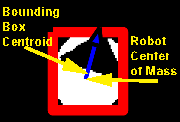
\includegraphics[width=0.5\textwidth]{../Drawings/orientationAlgorithm.pdf}
	\caption{Connecting the center of mass of the robot to the bounding box centroid to determine the robot's orientation}
	\label{fig:orientation}
\end{figure}

The algorithm initially receives the center of mass coordinates of the robot as well as the bounding box centroid as shown in the code below. Using these values, the algorithm then defines vectors \textit{DR, DG} and \textit{DB} for each of the three colour channels. By normalising these vectors using \eqnref{eqn:norm}, unit vectors are obtained and are then scaled to create the arrows pointing in the direction of the robots current orientation. These arrows are then plotted on the current image frame using a third-party function called \textit{$plot\_arrow$}.\\

\begin{equation}
D_{x} = \frac{D_{x}}{\vert\vert D_{x} \vert\vert}
\label{eqn:norm}
\end{equation}

\lstinputlisting{unitVectorReport.m}

\subsection{Background Estimation}
\label{sec:back}
Estimation of the background image required the implementation of a variety of different image processing techniques. This is because the datasets provided presented a number of challenges. One such challenge was that of removing robots that were stationary for a significant portion of a frame sequence. This prevented the simple implementation of a median filter to calculate the background image. This is due to the fact that objects that are stationary for a large subset of the frames will be incorporated into the median and subsequently into the background image.\\

Therefore, in order to solve this problem, an algorithm has been developed to calculate the background image, regardless of stationary robots being in large subsets of the frame sequence. \\

The background estimation algorithm consists of three main functional blocks. These blocks are \textit{Channel Processing}, \textit{Region Erasing and Filling} and \textit{Median Filtering} respectively. The \textit{Channel Processing} block receives an image frame and processes the image. This includes blurring, normalising, separating the image into its three channels, subtracting the blue channel from the green channel and renormalising the image. This creates an image that is ready for \textit{Region Erasing and Filling}. In order to implement this functional block, the image channels for the current frame are input into a function called \textit{eraseRegion}. A code snippet of the function is shown below.\\

\lstinputlisting{eraseRegion.m}

This function calculates the average value of the pixels found at the corner vertices of the bounding boxes surrounding each robot as shown in \figref{fig:vertices}. The corner pixels are averaged across all three colour channels and are stored in the variable \textit{Avg}. All of the pixels in the region containing the robot are then filled with this new average value to produce the image shown in \figref{fig:vertices}. This is applied to each of the robots in the image. \\

\begin{figure}[h!]
	\centering
		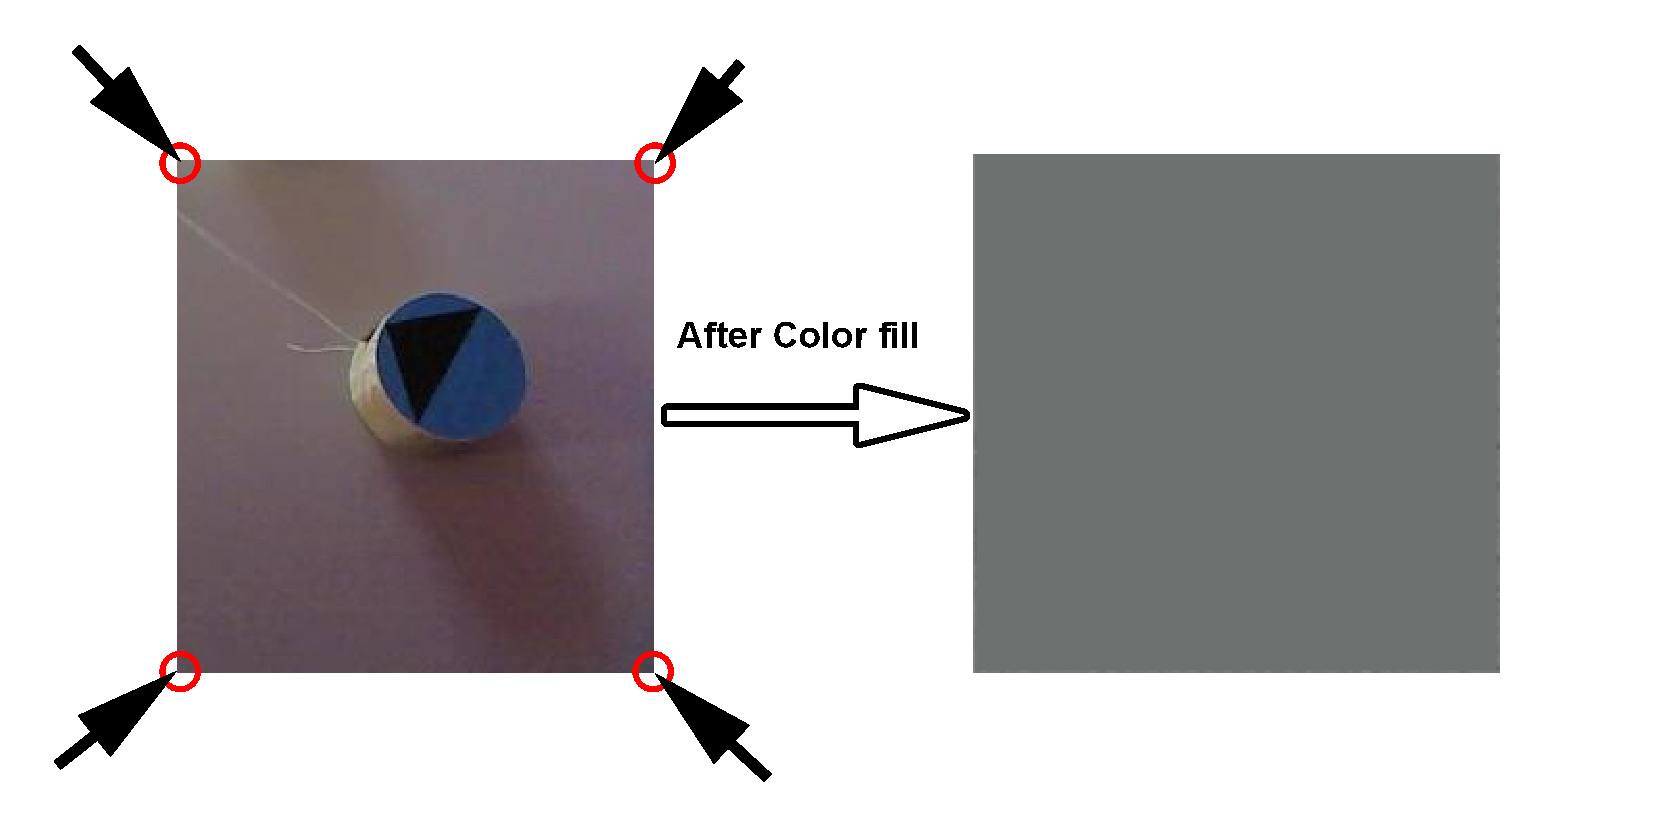
\includegraphics[width=0.8\textwidth]{../Drawings/backgroundErasingMain.pdf}
	\caption{The corner pixel intensities are averaged and are then used to fill the region of the image containing the robot}
	\label{fig:vertices}
\end{figure}

The \textit{Region Erasing and Filling} functional block is implemented on the three image frames that are used for background estimation. The reason three image frames have been chosen is because this is the minimum number of frames required to effectively use a median filter which is utilised in the \textit{Median Filtering} functional block. In addition to this, using a small number of frames to compute the median minimises the algorithm's processing time. The median of the three images is subsequently computed to produce an estimation of the background image.

\section{Results}
\label{sec:results}
Test data
\subsection{Robot Detection}
\label{sec:detect}


\begin{table}[ht]
\caption{Results obtained from trying to detect whether or not a robot is in an image frame} 
\centering 
\begin{tabular}{|c|c|c|c|c|c|c|c|c|c|} 
\hline
 & \multicolumn{3}{c} {Dataset 1}&\multicolumn{3}{c} {Dataset 8}&\multicolumn{3}{c} {Dataset 10}\\
\hline
Type &Red & Green & Blue & Red & Green & Blue &Red &Green &Blue \\ 
\hline
Correct Detection	& 73 & 91 & 95 & 95 & 95  &95 &95 &95 &95 \\
Missed Detection	& 0  & 0  & 0  & 0  & 0   &0  &0  &0  &0  \\
Incorrect Detection & 22 & 4  & 0  & 0  & 0   &0  &0  &0  &0 \\
\hline %inserts single line
\end{tabular}
\label{table:detection}
\end{table} 

An example of an incorrect detection of a robot due to the robot leaving the image frame.
\begin{figure}[h!]
\begin{minipage}[b]{0.5\linewidth}
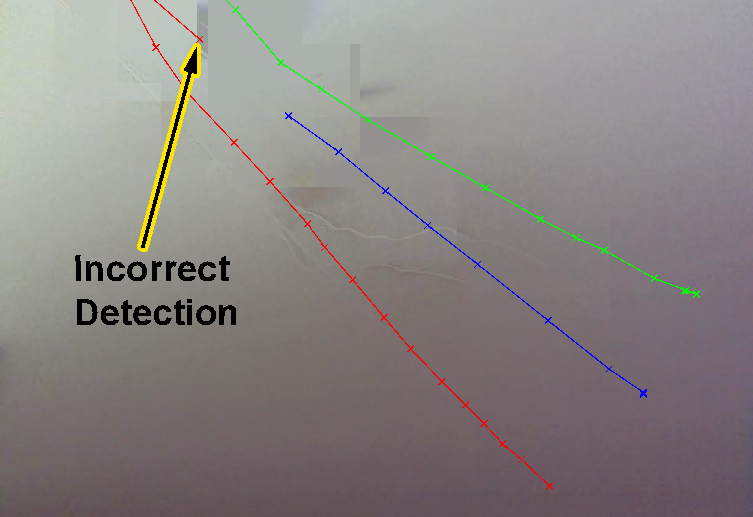
\includegraphics[scale=0.5]{../Drawings/incorrectdetBackdata1.pdf}
\caption{An incorrect detection of the red robot. This track has been linked to the track of the blue robot creating an incorrect track.}
\label{fig:InDetectData2}
\end{minipage}
\hspace{0.5cm}
\begin{minipage}[b]{0.5\linewidth}
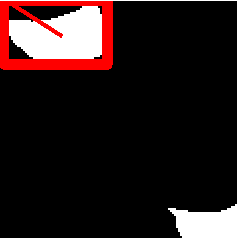
\includegraphics[scale=0.8]{../Drawings/incorrectdetrobotdata1.pdf}
\caption{The incorrect detection of the red robot as shown in the red channel binary image.}
\label{fig:redInDetect}
\end{minipage}
\end{figure}

An example of an incorrect detection of a robot due to a region of highly saturated pixels that have a similar colour to that of the robot.

\begin{figure}[h!]
\begin{minipage}[b]{0.5\linewidth}
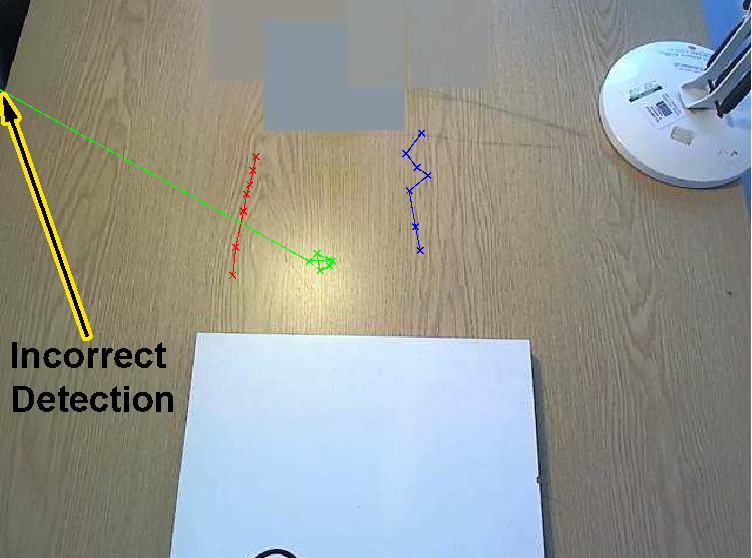
\includegraphics[scale=0.5]{../Drawings/incorrectdetBackdata7.pdf}
\caption{An incorrect detection of the green robot. This results in a broken track}
\label{fig:InDetectData7}
\end{minipage}
\hspace{0.5cm}
\begin{minipage}[b]{0.5\linewidth}
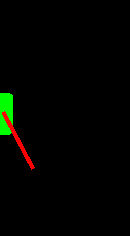
\includegraphics[scale=0.8]{../Drawings/incorrectdetrobotdata7.pdf}
\caption{The incorrect detection of the green robot due to a small region of highly saturated pixels. }
\label{fig:greenInDetect}
\end{minipage}
\end{figure}

\subsection{Linking Robot Tracks}
\label{sec:linking}
As detailed in \secref{sec:linking}, a linking algorithm for the robots has been developed. This algorithm was tested on a variety of datasets and the results are tabulated in \tabref{table:linking}. This table details the number of \textit{Correct tracks, Incorrect Tracks} and \textit{Broken Tracks}. A \textit{Broken Track} has been defined as a connection between two tracks whereby the latter track is an incorrect detection of a robot. \\

The linking algorithm performed well on dataset $8$ and dataset $10$. However, dataset $1$ had a large number of incorrect and broken tracks, especially on the red channel. These errors occurred as a result of the red robot leaving the image frame. As the robot leaves the frame, the algorithm looks for a set of red pixels that correspond to a red robot. Since the robot is not present, the algorithm identifies the next largest area of red pixels as being the red robot. This is incorrect and causes the results below.\\

An example of this is shown in \figref{fig:InDetectData2} and \figref{fig:redInDetect}. In this example, the red robot has left the scene and a group of red pixels, as shown in \figref{fig:redInDetect}, have been incorrectly defined as being the red robot. This results in an incorrect linkage between two tracks.

\begin{table}[ht]
\caption{Results obtained from linking robot tracks on a variety of different datasets} 
\centering 
\begin{tabular}{|c|c|c|c|c|c|c|c|c|c|} 
\hline
 & \multicolumn{3}{c} {Dataset 1}&\multicolumn{3}{c} {Dataset 8}&\multicolumn{3}{c} {Dataset 10}\\
\hline
Type &Red & Green & Blue & Red & Green & Blue &Red &Green &Blue \\ 
\hline
Correct Tracks	 & 73 & 91 & 95 & 95 & 95  &95 &95 &95 &95 \\
Incorrect Tracks & 10 & 2  & 0  & 0  & 0   &0  &0  &0  &0  \\
Broken Tracks    & 12 & 2  & 0  & 0  & 0   &0  &0  &0  &0 \\
\hline %inserts single line
\end{tabular}
\label{table:linking}
\end{table} 

Another situation occurs whereby the robot tracks are incorrectly linked. As seen in \figref{fig:InDetectData7}, the green robot track has been incorrectly linked to the left hand side of the image frame. 
%Check the cause of this problem.

\begin{figure}[h!]
	\centering
		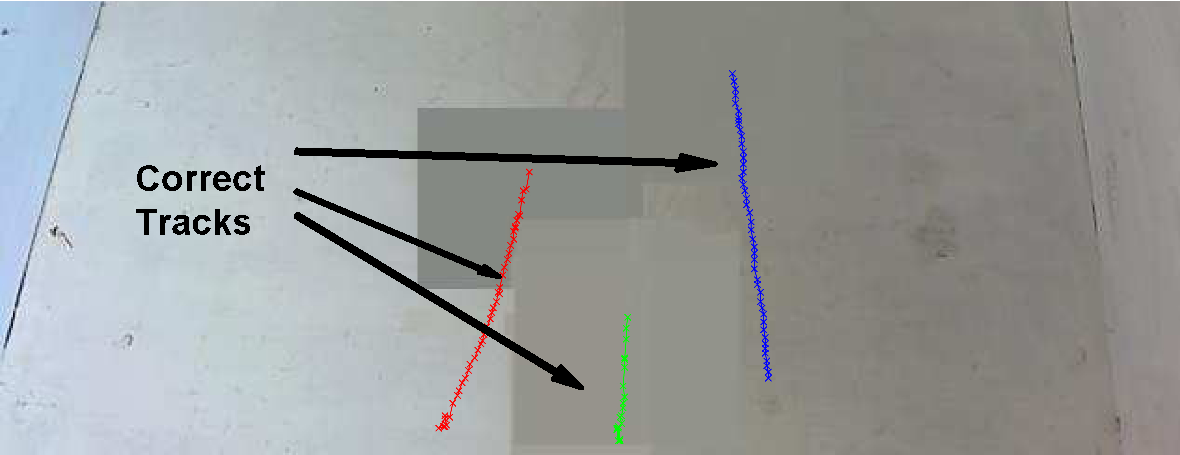
\includegraphics[width=0.6\textwidth]{../Drawings/correctTracksData8.pdf}
	\caption{An example of correct robot tracks}
	\label{fig:tracks}
\end{figure}


\subsection{Robot Orientation}
\label{sec:orient}
The orientation of the robots was tested on a variety of different datasets and the results for each dataset is presented in \tabref{table:direction}. It has been found that it is generally possible to determine the orientation of the robot. However, there are a number of scenarios whereby the orientation is incorrectly determined causing the arrowheads to point in incorrect directions. 

\begin{table}[ht]
\caption{Results obtained from determining which direction the robot is facing} 
\centering 
\begin{tabular}{|c|c|c|c|c|c|c|c|c|c|} 
\hline
 & \multicolumn{3}{c} {Dataset 1}&\multicolumn{3}{c} {Dataset 8}&\multicolumn{3}{c} {Dataset 10}\\
\hline
Type &Red & Green & Blue & Red & Green & Blue &Red &Green &Blue \\ 
\hline
Missed Direction	& 6  & 6 & 2 & 0 & 0  &0  &0 &2 &4 \\
Incorrect Direction	& 0  & 6 & 0 & 1 & 11 &3  &4 &12 &2  \\
Correct Direction 	& 89 & 83& 93& 94& 84 &92 &91 &81 &89 \\
\hline %inserts single line
\end{tabular}
\label{table:direction}
\end{table}  

  \begin{figure}[h!]
	\centering
		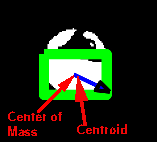
\includegraphics[width=0.5\textwidth]{../Drawings/IncorrectDirectionResults.pdf}
	\caption{Examples of correct, incorrect and missed arrow orientations respectively}
	\label{fig:indetect}
\end{figure}

An example of incorrect and missed orientation in an image frame.

\begin{figure}[h!]
	\centering
		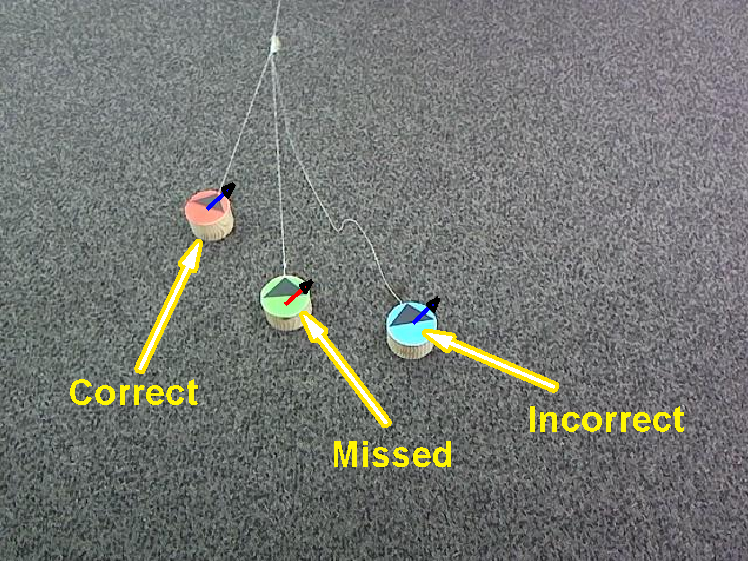
\includegraphics[width=0.5\textwidth]{../Drawings/missedandIncorrectDetData2Ready.pdf}
	\caption{Examples of correct, incorrect and missed arrow orientations respectively}
	\label{fig:indetect}
\end{figure}


\subsection{Background Images}
\label{sec:back}
An example of background images produced using the Background Estimation Algorithm detailed in \secref{sec:back}.

\begin{figure}[h!]
\begin{minipage}[b]{0.5\linewidth}
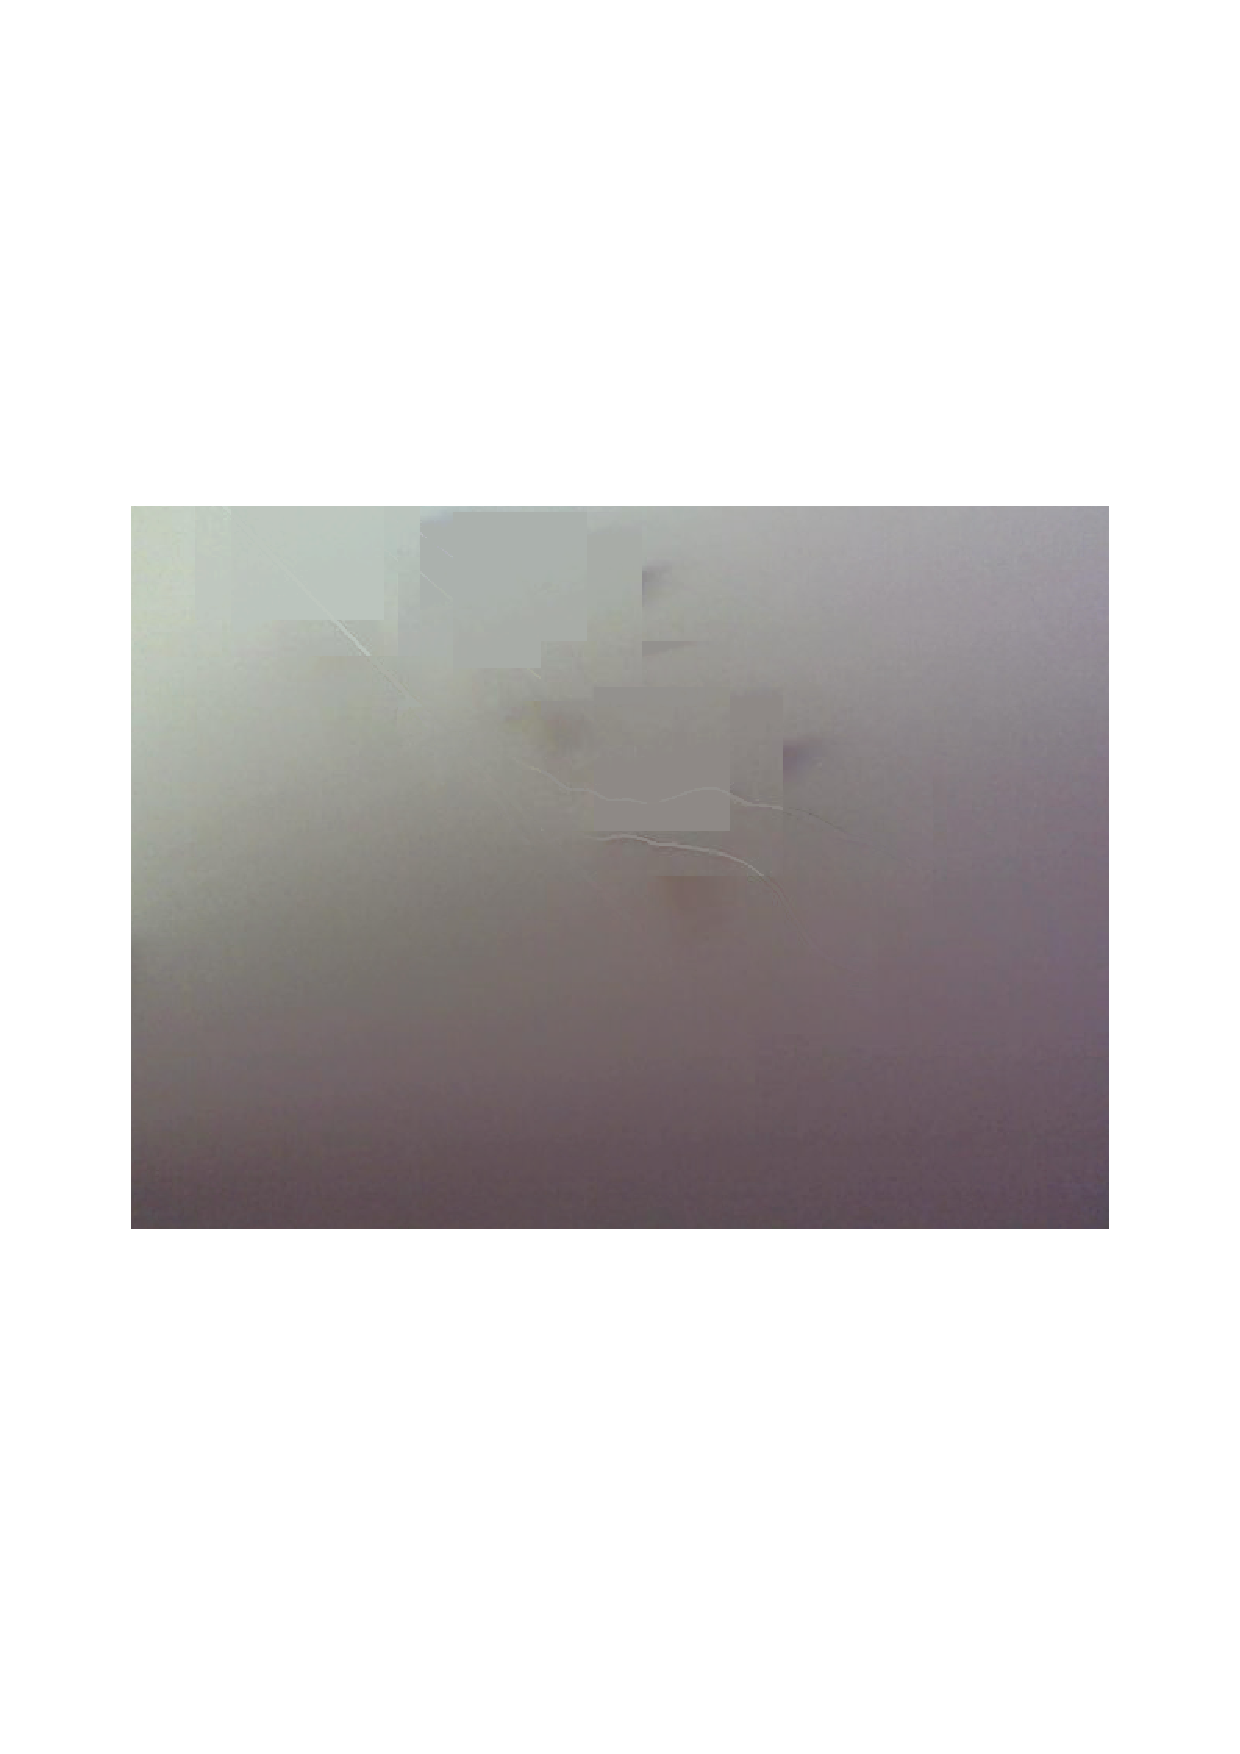
\includegraphics[scale=0.4]{../Drawings/backdata1.pdf}
\caption{The estimated background image of the first dataset provided for image processing}
\label{fig:backdata1}
\end{minipage}
\hspace{0.5cm}
\begin{minipage}[b]{0.5\linewidth}
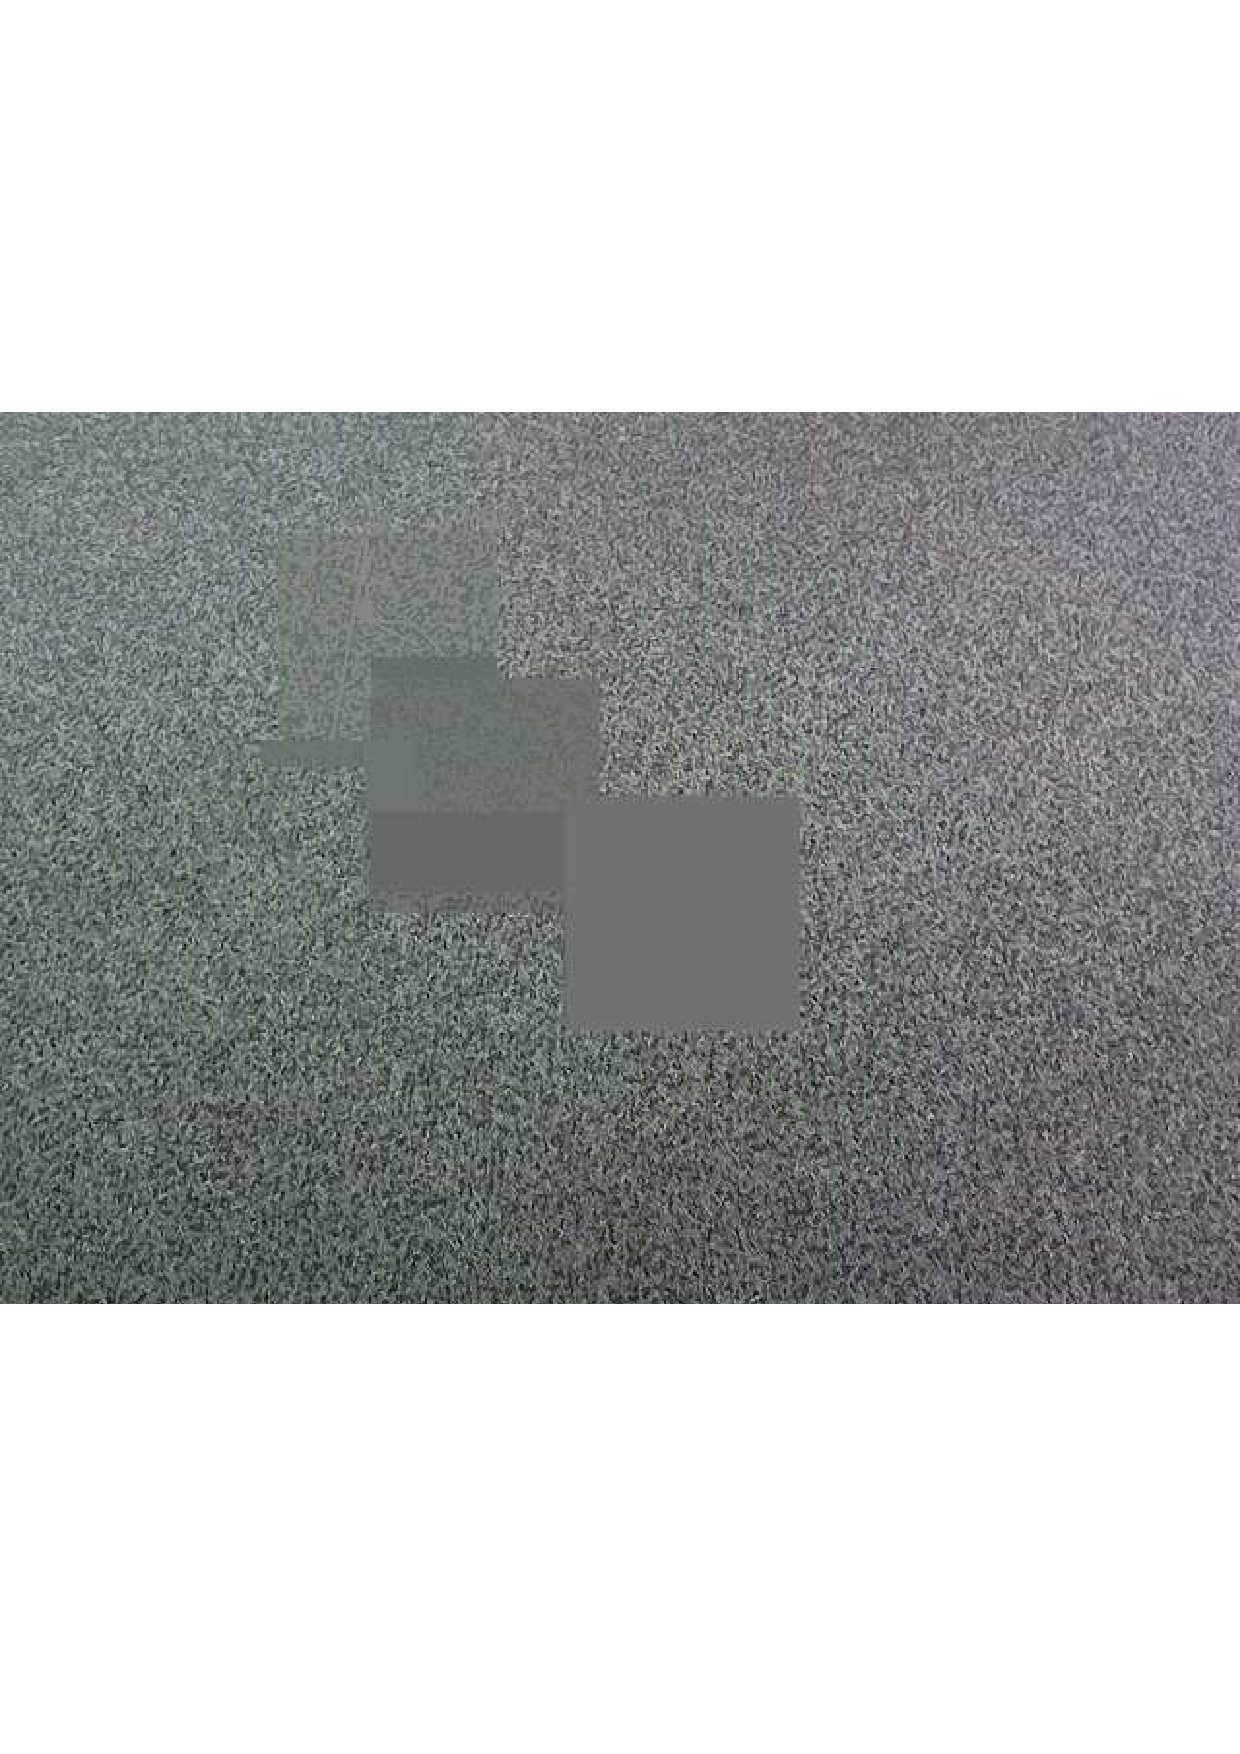
\includegraphics[scale=0.3]{../Drawings/backdata2.pdf}
\caption{The estimated background image of the second dataset provided for image processing}
\label{fig:backdata2}
\end{minipage}
\end{figure}


\begin{figure}[h!]
\begin{minipage}[b]{0.5\linewidth}
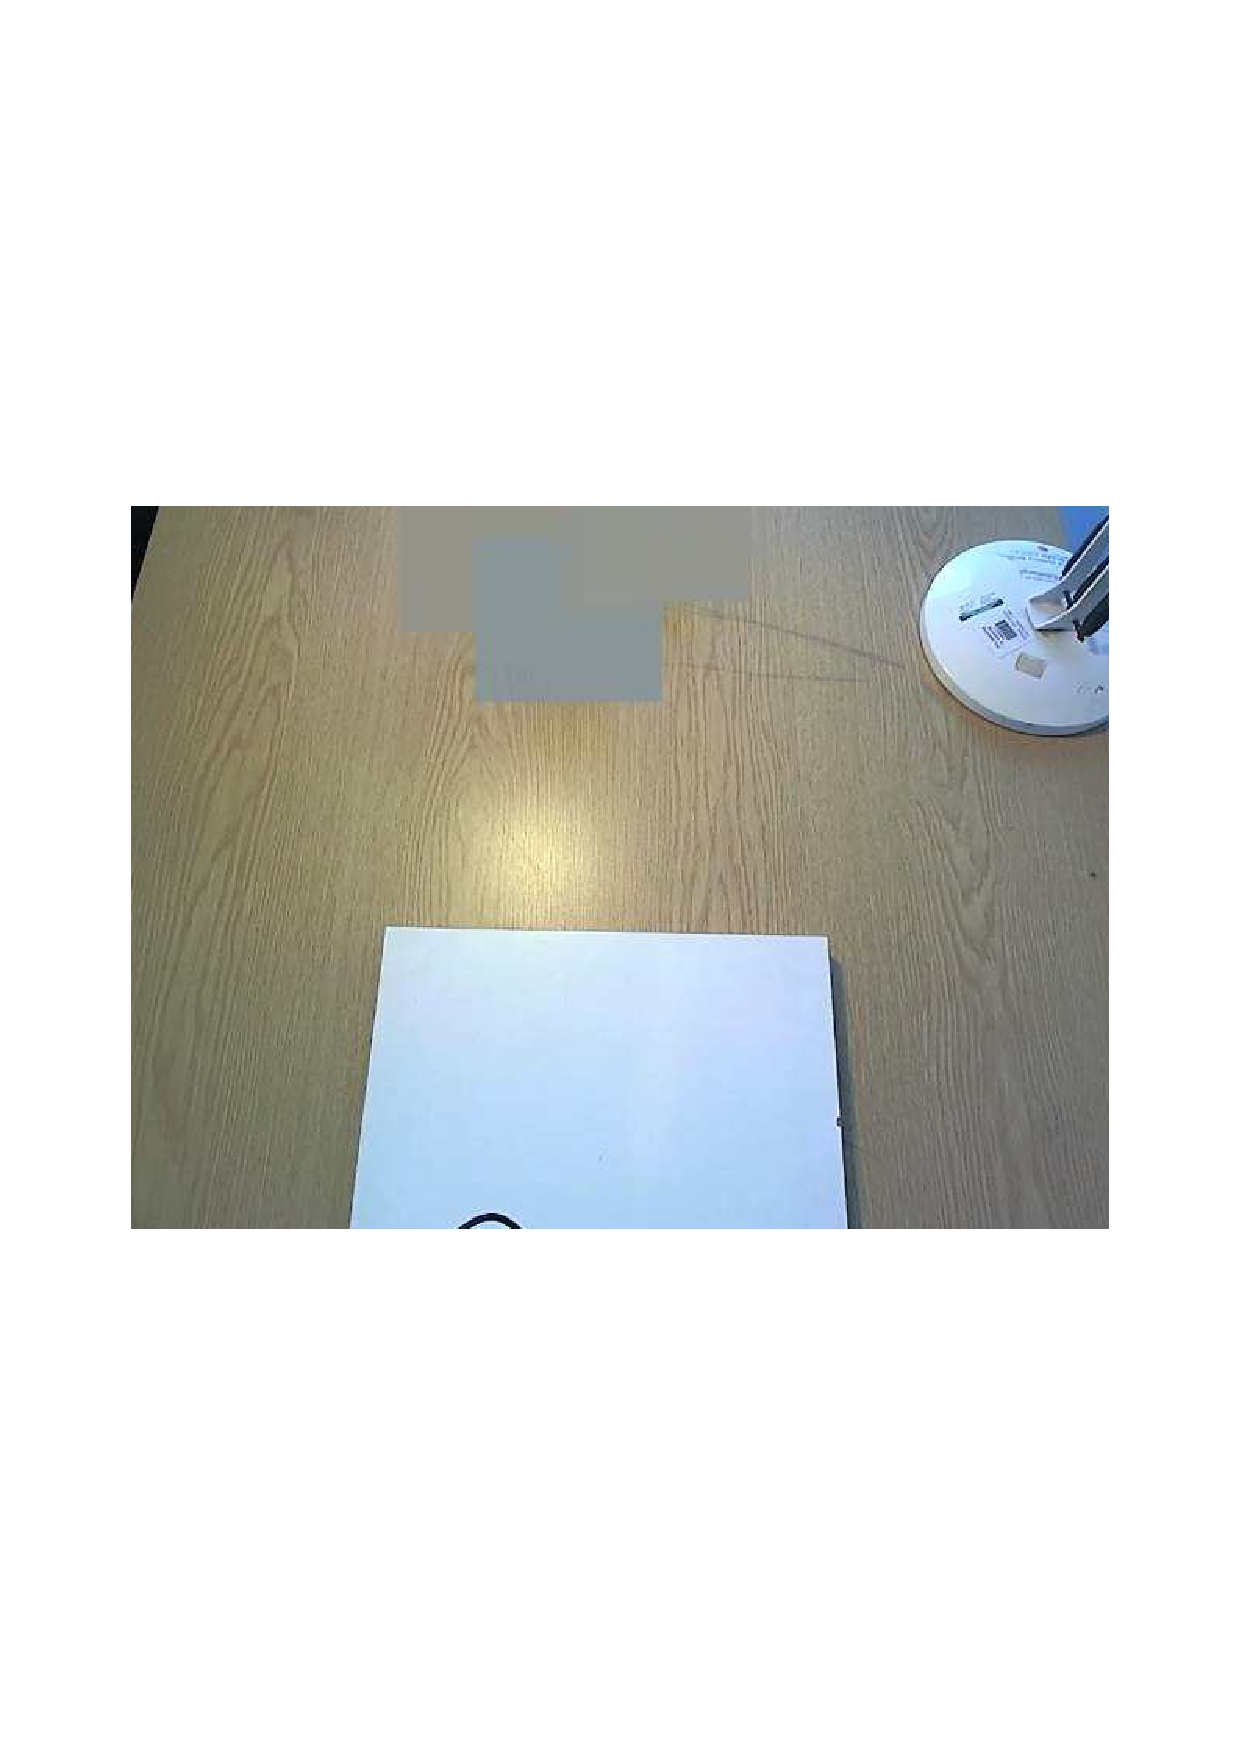
\includegraphics[scale=0.3]{../Drawings/backdata7.pdf}
\caption{The estimated background image of a new test dataset}
\label{fig:backdata7}
\end{minipage}
\hspace{0.5cm}
\begin{minipage}[b]{0.5\linewidth}
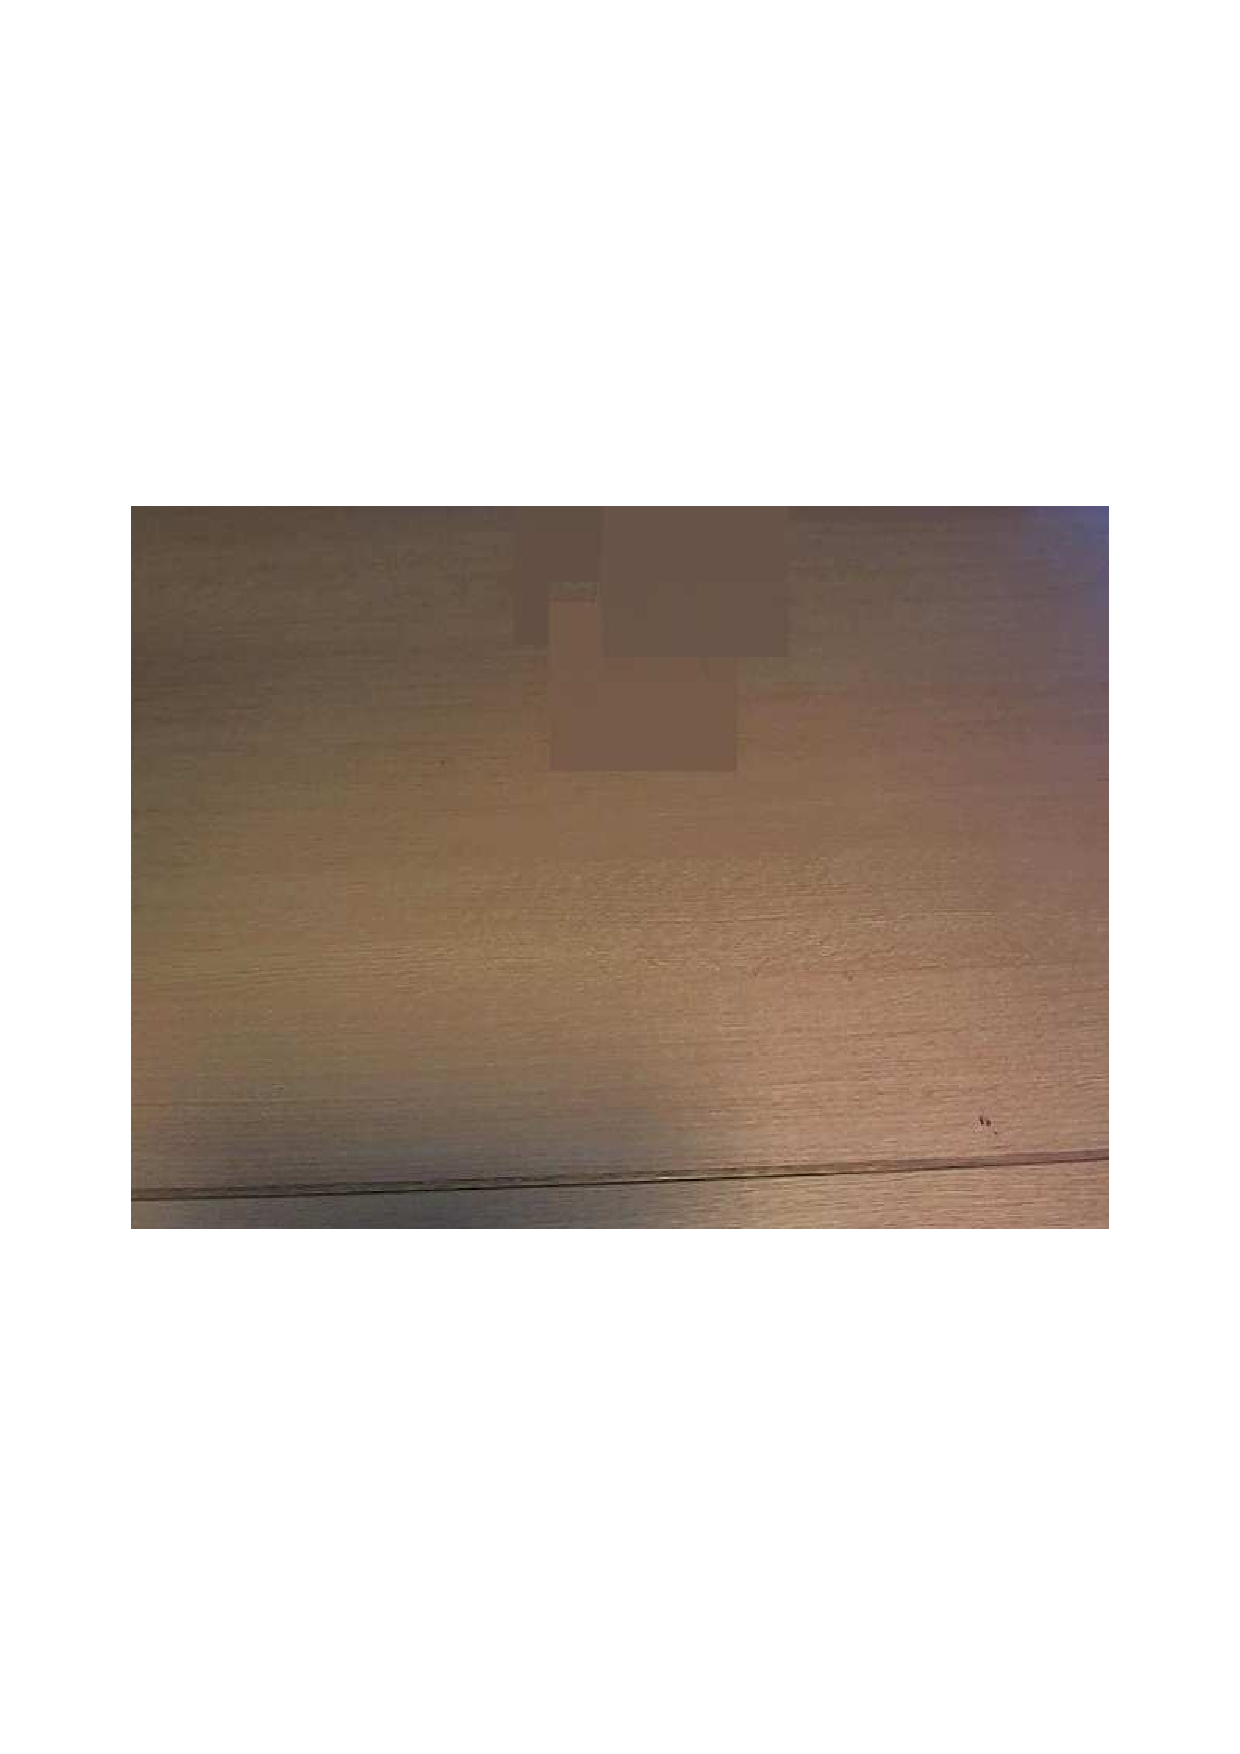
\includegraphics[scale=0.3]{../Drawings/backdata10.pdf}
\caption{The estimated background image of a new test dataset}
\label{fig:backdata10}
\end{minipage}
\end{figure}

%Show an example of results for each stage of detection

\section{Discussion}
\label{sec:discussion}
Assess the success of the program with regard to:

%1. Report results

%Discuss any
%1. Limitations, problems
%2. Improvements you would make

\section{Code}
\label{sec:code}
%Any downloaded code should be recorded in the report. Does not need to be in the appendix
%Code from course web pages are not needed

\section{Conclusion}
\label{sec:conclusion}

%\bibliographystyle{witseie}
%\bibliography{bibliography}
 \newpage
\onecolumn
\appendix
\setcounter{table}{0}
\setcounter{figure}{0}
\setcounter{subsection}{0}
\makeatletter \renewcommand{\thefigure}{A.\@arabic\c@figure} \renewcommand{\thetable}{A.\@arabic\c@table} \renewcommand{\thesection}{A.\@arabic\c@section} \makeatother
\section*{APPENDIX A}

\section{Control Program}
%Add the matlab code to this file...
%\lstinputlisting{codeSnippets.cpp}
 
\end{document}

